\documentclass[11pt]{article}


\usepackage{multicol}
\usepackage{natbib}
\usepackage{pdfpages}
\usepackage{tikz}
\usepackage{amsmath}
\usepackage{amsfonts}
\usepackage{url}

\Urlmuskip=0mu plus 1mu


\setlength{\hoffset}{0pt}
\setlength{\voffset}{0pt}
\setlength{\oddsidemargin}{0pt}
\setlength{\topmargin}{0pt}
\setlength{\topsep}{0pt}
\setlength{\headsep}{0pt}
\setlength{\headheight}{0pt}
\setlength{\textwidth}{6.5in}
\setlength{\textheight}{9in}

% \newcommand{\solutionname}{[Solution Name]}
\newcommand{\organization}{TeMa}
\newcommand{\solutiontitle}{Empirical Inference of Underlying Condition Probabilities Using Synthea-Generated Synthetic Health Data}
\newcommand{\challengecategory}{II (Novel Uses of Synthea Generated Synthetic Data)}
\newcommand{\ABSTRACT}{Diagnosing an ailment is essentially a Bayesian problem; a doctor only knows what she can observe and must use this information to infer the patient's condition.  In this effort, we provide a prototype implementation that uses Synthea-generated synthetic electronic health records (EHRs) to study the complicated relationships between sets of symptoms and the likelihoods of possible underlying causes.  The goal of this work is to determine the most likely patient pathologies based on a given set of observed symptoms and patient demographics. We apply two distinct methods aimed at achieving this goal.  Our first method relies on a strictly empirical analysis of synthetic EHRs to obtain posterior pathology probabilities.  Our second approach uses the synthetic EHRs to populate probability distribution functions in a graph-based machine learning model.  We give a qualitative and quantitative comparison of these two methods.  Finally, we show how we validated these models, demonstrate how they can be used as a mechanism for validating the outputs of Synthea, and suggest promising research applications of the methods we have proposed.
}


\begin{document}

%%% COVER PAGE

\thispagestyle{empty}

~
\vspace{\stretch{1}}

\begin{center}
    {\huge \solutiontitle} \\[24pt]
    {\Large Submission for the Synthetic Health Data Challenge} \\[24pt]
    {\Large By:} \\[24pt]
\end{center}

\begin{multicols}{2}
\begin{center}
	Michael D. Teter\\
	miketeter@yahoo.com
\end{center}

\columnbreak

\begin{center}
    Christopher E. Marks\\
    pb2pv@yahoo.com
\end{center}
\end{multicols}

\vspace{\stretch{0.2}}


\noindent \textbf{Challenge Category:} \challengecategory
\\

\vspace{\stretch{1}}

\clearpage

%% Body %%

\setcounter{page}{1}

\begin{center}
  {\LARGE \solutiontitle}
  \\[11pt]
  \begin{minipage}{0.9\textwidth}
    \textbf{Abstract:}
    \ABSTRACT
  \end{minipage}
\end{center}


\section{Overview} \label{sec: overview}

Patient diagnosis is fundamental to good health care.  In this research effort, we investigate a Bayesian approach to patient diagnosis, using data generated by Synthea. Our immediate goal is to construct models that input a set of symptoms, and based on a large set of synthetic EHRs, output the set of most likely causes.  This analytic workflow is similar to how a doctor might arrive at a diagnosis: he mentally follows a flow model based on his understanding of the most probable causes of the symptoms he observes.  Analysis of the statistical distributions of symptoms and diseases in Synthea data could assist in validating the diagnosis work flows used in practice and add mathematical rigor to the intuition doctors develop through education and experience.  The methods we employ could be extended to include other relationships in Synthea data in order to gain insights that generalize to a wide variety of applications.

%%%%%%%%% FIGURE %%%%%%%%%%%%

\begin{figure}[!bth] \centering
  \begin{tikzpicture}[scale=0.5]
  \node[anchor=east] at (0,0){\scriptsize Patient};
  \path[draw] (0,0) node(n0){} -- (5,4)
    node[midway,above,rotate=38.66]{\scriptsize $p=0.005$} 
    node[midway,below,rotate=38.66](b){\scriptsize Bronchitis}
    node(bronch){};
  \path[draw] (0,0) node(n0){} -- (5,-4)
    node[midway,above,rotate=-38.66]{\scriptsize $p=0.0058$} 
    node[midway,below,rotate=-38.66](st){\scriptsize Sore Throat}
    node(sorethroat){};
  \path[draw] (5,4) -- (10,7) 
    node(f0)[pos=0.66,above,rotate=30.96]{\scriptsize $s \sim U(25,50)$}
    node(f0)[pos=0.66,below,rotate=30.96]{\scriptsize \textbf{Fever}};
  \path[draw] (5,4) -- (10,4) 
    node(f0)[pos=0.99,above]{\scriptsize $s \sim U(25,50)$}
    node(f0)[pos=0.99,below]{\scriptsize Nasal cong.};
  \path[draw] (5,4) -- (10,1) 
    node(f0)[pos=0.80,above,rotate=-30.96]{\scriptsize $s \sim U(0,25)$}
    node(f0)[pos=0.80,below,rotate=-30.96]{\scriptsize Body aches};
  \path[draw] (5,-4) -- (10,-2) 
    node(f0)[pos=0.66,above,rotate=21.8]{\scriptsize $s \sim U(0,50)$}
    node(f0)[pos=0.66,below,rotate=21.8]{\scriptsize \textbf{Fever}};
  \path[draw] (5,-4) -- (10,-6) 
    node(f0)[pos=0.66,above,rotate=-21.8]{\scriptsize $s \sim U(0,50)$}
    node(f0)[pos=0.66,below,rotate=-21.8]{\scriptsize Body aches};
  \node[anchor=west] at (10,7){\scriptsize $p \cdot f_{s}(35) = 0.005 \cdot \frac{1}{25} = \mathbf{0.0002}$};
  \node[anchor=west] at (10,-2){\scriptsize $p \cdot f_{s}(35) = 0.0058 \cdot \frac{1}{50} = \mathbf{0.000116}$};
  \end{tikzpicture}
  \caption{Conditional probability diagram for select symptoms related to bronchitis, sinusitis, and sore throat. \label{fig: condprob}}
  \end{figure}
  
  %%%%%%%%% END FIGURE %%%%%%%%


Simulations such as Synthea can be used to investigate the complicated probabilistic relationships for which exact analytic derivations are intractable.  Synthea \citep{walonoski2018synthea} consists of a configurable set of modules, each of which stochastically generates medical conditions and associated symptoms. For example, a patient under 18 years old has a 0.5\% chance of developing bronchitis each month, and \emph{given the patient has developed bronchitis}, the conditional probability the patient develops a fever is 1 \citep{bronchitisModule}.  The probabilities encoded in Synthea's modules are based on known characteristics and incidence rates of various pathologies and conditions.

It somewhat difficult, however, to analytically determine the combined probability that a patient develops a fever for any reason.  It requires even more work to determine the conditional (posterior) probability, \emph{given the patient has a fever}, that the underlying cause is bronchitis.  The analysis gets even more complicated if we also account for symptom severity, patient demographics, or other factors.  Figure \ref{fig: condprob} depicts a simple conditional probability diagram for the ``Fever'' and "Body aches" symptoms associated with just two of the Synthea modules.  The figure includes the severity distributions for the depicted symptoms, where $U$ denotes the uniform distribution.  Synthea's workflows essentially move from left to right in Figure \ref{fig: condprob} to generate pathologies and then symptoms.  Our task (and the task of doctors diagnosing patients) is to infer the pathology from the symptoms and severities, working instead from the right side of Figure \ref{fig: condprob} to the left.


\section{Methods}

We introduce and implement two techniques for using Synthea data to find posterior probabilities for pathologies, given a set of symptoms and basic patient demographics.  The first method is to use Synthea's output to perform a strictly empirical Bayesian analysis.  The second method applies graphical models from machine learning literature (see, e.g., \cite[pp 359--383]{bishop2013pattern}) to obtain similar, but potentially more generalizable results.

\subsection{Empirical Bayesian Analysis} \label{section: empirical-analysis}

Suppose we have a notional 5 year old female patient presenting with a fever, and we want to know the potential underlying pathologies and their associated probabilities.  Using a large set of Synthea-generated ``symptoms'' records, we can query those that contain the "fever" symptom for a 5 year old female, and from this subset investigate the different underlying causes and their associated frequencies. Figure \ref{fig: fever-pathologies} depicts the posterior probabilities of the five most likely pathologies (out of ten total) that result from applying this method on a set of 5000 Synthea-generated patients.

\begin{figure}[!hbt]\centering
  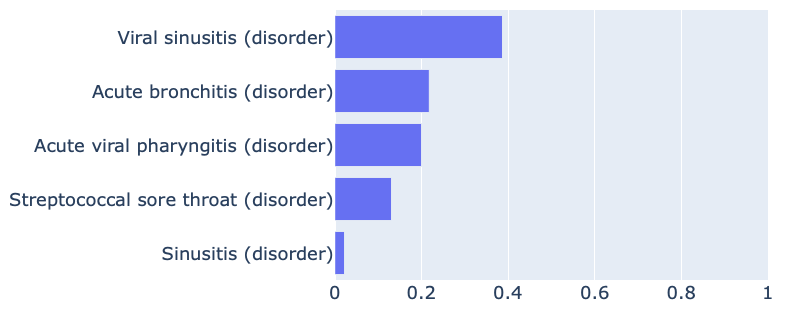
\includegraphics[width=0.75\textwidth]{figures/fever-pathologies.png}
  \caption{The five most common pathologies presenting the ``Fever'' symptom, and their associated probabilities. \label{fig: fever-pathologies}}
\end{figure}

What about the severity of the fever?  Again we can use Synthea data to perform an empirical analysis.  Figure \ref{fig: fever-severity} shows the empirically derived conditional probability density functions associated with each of the most likely pathologies for the ``Fever'' symptom.  Notice that neither ``Viral sinusitis'' nor ``Acute bacterial sinusitis'' are likely to produce a fever with severity level higher than 25 (per Synthea's severity encoding), while ``Acute bronchitis'' is unlikely to produce a fever with a low severity.  If we had additional information on the severity of the fever, we could use this analysis to provide additional insights, and further update posterior probabilities. 

\begin{figure}[!hbt]\centering
  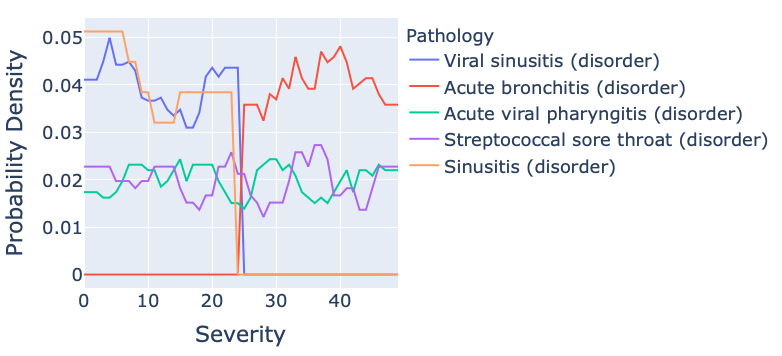
\includegraphics[width=0.75\textwidth]{figures/fever-severity.png}
  \caption{Fever severity distributions for most likely pathologies. \label{fig: fever-severity}}
\end{figure}

There is some risk, however, of obtaining too few results when using this strictly empirical Bayes analysis method.  A query for records of a 5 year old girl with a fever resulting from ``Sinusitis (disorder)'' returns only 18 results out of 315,729 rows in our underlying Synthea-generated symptoms data.  To generate the fever severity density function plotted in Figure \ref{fig: fever-severity} from these 18 points, we used a $k$-nearest neighbor algorithm and normalized the resulting function so that it summed to one. The Bayesian network approach described in the next section mitigates this problem by decoupling some of the variables in the analysis.  



\subsection{Bayesian Network Analysis}

This section builds on the empirical analysis discussed in the previous section, but employs a model that is easier to generalize.  As discussed, the strictly empirical analysis in the previous section can result in small sample sizes of limited utility.  We can overcome this limitation by making some assumptions on the dependencies between the variables we are analyzing.  Our assumptions are captured in the Bayesian network \citep[pp. 360--383]{bishop2013pattern} model depicted in Figure \ref{fig: graphs}(a), in which the directed edges imply probabilistic dependence between two variables.  If two variables (represented as nodes in Figure \ref{fig: graphs}(a)) are not connected by an edge, they are conditionally independent, i.e., they become independent when the values for the nodes between them are known.  

For example, we assume that pathology probabilities depend on a patient's age and gender, but symptoms and symptom severities (abbreviated as $S_{x}$ and $V_{x}$ in Figure \ref{fig: graphs}(a), respectively) \emph{do not} depend on age and gender once the pathology is known.  Of course there are cases where this assumption does not hold, but it provides a useful simplification for the reasons discussed.

\begin{figure}[!htb]\centering
  \begin{tabular}{c@{\hspace{3em}}c} 
\begin{tikzpicture}[scale=0.6]
\node(gender)[circle,draw] at (0,2){\scriptsize Gender};
\node(age)[circle,draw] at (0,-2){\scriptsize Age};
\node(pathology)[circle,draw] at (3,0){\scriptsize Pathology};
\node(s1)[circle,draw] at (6,6){\scriptsize $S_{1}$};
\node(v1)[circle,draw] at (6,3.5){\scriptsize $V_{1}$};
\node(s2)[circle,draw] at (6,1.5){\scriptsize $S_{2}$};
\node(v2)[circle,draw] at (6,-1){\scriptsize $V_{2}$};
\node(vdots) at (6,-2) {\vdots};
\node(sn)[circle,draw] at (6,-3.5){\scriptsize $S_{N}$};
\node(vn)[circle,draw] at (6,-6){\scriptsize $V_{N}$};
\path[draw,-latex] (gender) -- (pathology);
\path[draw,-latex] (age) -- (pathology);
\path[draw,-latex] (pathology) -- (s1);
\path[draw,-latex] (pathology) -- (v1);
\path[draw,-latex] (s1) -- (v1);
\path[draw,-latex] (pathology) -- (s2);
\path[draw,-latex] (pathology) -- (v2);
\path[draw,-latex] (s2) -- (v2);
\path[draw,-latex] (pathology) -- (sn);
\path[draw,-latex] (pathology) -- (vn);
\path[draw,-latex] (sn) -- (vn);
\end{tikzpicture}
& 
% \caption{Bayesian network model of pathologies and symptoms. \label{fig: bayesian-network}}
% \end{figure}
% \columnbreak
% \begin{figure}[!hbt]\centering
\begin{tikzpicture}[scale=0.6]
\node(gender)[circle,draw] at (0,2){\scriptsize Gender};
\node(age)[circle,draw] at (0,-2){\scriptsize Age};
\node(gap)[rectangle,draw] at (2.5,0){\scriptsize GAP};
\node(pathology)[circle,draw] at (5,0){\scriptsize Pathology};
\node(s1)[circle,draw] at (10,5){\scriptsize $S_{1}$};
\node(v1)[circle,draw] at (10,3){\scriptsize $V_{1}$};
\node(pss1)[rectangle,draw] at (7.5,4){\scriptsize $PSS_{1}$};
\node(s2)[circle,draw] at (10,1){\scriptsize $S_{2}$};
\node(v2)[circle,draw] at (10,-1){\scriptsize $V_{2}$};
\node(pss2)[rectangle,draw] at (7.5,0){\scriptsize $PSS_{2}$};
\node(vdots) at (10,-2.25) {\vdots};
\node(sn)[circle,draw] at (10,-4){\scriptsize $S_{N}$};
\node(vn)[circle,draw] at (10,-6.5){\scriptsize $V_{N}$};
\node(pssn)[rectangle,draw] at (7.5,-4){\scriptsize $PSS_{N}$};
\path[draw,-] (gender) -- (gap);
\path[draw,-] (age) -- (gap);
\path[draw,-] (gap) -- (pathology);
\path[draw,-] (pathology) -- (pss1);
\path[draw,-] (pss1) -- (s1);
\path[draw,-] (pss1) -- (v1);
\path[draw,-] (pathology) -- (pss2);
\path[draw,-] (pss2) -- (s2);
\path[draw,-] (pss2) -- (v2);
\path[draw,-] (pathology) -- (pssn);
\path[draw,-] (pssn) -- (sn);
\path[draw,-] (pssn) -- (vn);
\end{tikzpicture}
\\[12pt]
(a) Bayesian network. &
(b) Factor graph.
\\
\end{tabular}
\caption{Bayesian network model (a) and corresponding factor graph (b). \label{fig: graphs}}
\end{figure}

We implemented the Bayesian network as a factor graph \citep[pp. 399--402]{bishop2013pattern}, as depicted in Figure \ref{fig: graphs}(b), to support efficient analysis, where factors are depicted as rectangular nodes and variables are circular.  The factor functions are:
\begin{itemize}
  \item GAP: $f(g,a,p) = p(g,a,p)$, i.e., the joint probability of a gender-age-pathology ($g,a,p$) combination, empirically derived from Synthea-generated data.
  \item $PSS_{i}$: $f(p,s_{i},v_{i}) = p(s_{i}|p)p(v_{i}|s_{i},p)$, i.e., the joint probability of a symptom-severity ($s_{i},v_{i}$) combination conditioned on pathology $p$, empirically derived from Synthea-generated data.
\end{itemize}
We can fix any subset of the variables in the factor graph and efficiently compute the conditional probability distributions for the remaining variables using the sum-product algorithm \citep[pp.402--411]{bishop2013pattern}.  

Using the Bayesian network method to investigate the likely causes for a 5 year old female with a fever produces the same results shown in Figure \ref{fig: fever-pathologies}.  This result is not surprising, as our Bayesian network model captures the dependencies between age, gender, and pathology.  However, the fever severity plot (Figure \ref{fig: bayes-fever-severity}) is smoother because, as a result of the decoupling induced by conditional independence, it makes use of all instances of fever in the data, and not only those in 5 year old females.

\begin{figure}[!hbt]\centering
  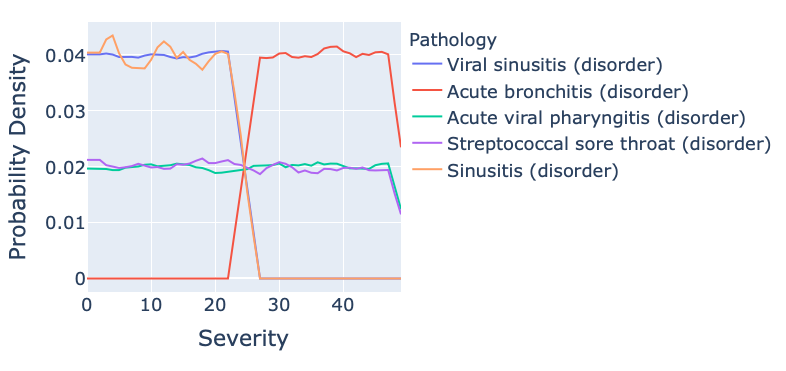
\includegraphics[width=0.75\textwidth]{figures/bayes-fever-severity.png}
  \caption{Bayesian network fever severity distributions. \label{fig: bayes-fever-severity}}
\end{figure}

%%%%%%%%%%%%%%%%%%%%%%%%%%%%%%%%%%%%%%%

\section{Implementation and Performance}

We provide a minimal application (https://github.com/teterholdings/Synthea\_Symptoms) that enables a user to select a set of symptoms, a patient age, patient gender, and the analysis method (empirical or Bayesian network).  The application executes the selected method to find the most likely pathologies and associated posterior probabilities.  Selected symptoms and resulting pathologies can be analyzed in more detail by following subsequent links.  In each case, the application carries out all of the analyses using the selected method.  When multiple symptoms are selected, the app conducts the analysis assuming all symptoms are simultaneously present and result from the same underlying cause.  As a result, many combinations of symptoms return no results because they are unlikely to occur together due to a single pathology.

The Bayesian network analyses take about 1-3 minutes, which is considerably longer than the empirical analysis of Section \ref{section: empirical-analysis} because of the computational resources required to build the factor graph and propagate the sum-product algorithm to all nodes.  

\section{Validation}

We provide two perspectives on validation.  First, we investigate whether our models, and specifically our factor graph implementation, are correctly capturing the marginals in the underlying data.  The second, more important aspect of validation deals with the underlying data and checks on the overall utility of using Synthea data in this way.

\subsection{Factor Graph Validation}

Because the sum-product algorithm requires careful curation of processing and memory, we developed some simple tests to validate its performance.  If we fix any combination of variables in the graph, the marginal probabilities for each of the remaining variables should sum to the frequency of that combination in the underlying Synthea data.  For example, suppose we fix the ``Gender'' variable in the factor graph (Figure \ref{fig: graphs}(b)) to be male.  After running the sum-product algorithm, the sum of the marginal probabilities for any other node (e.g., ``Cough'' symptom) should equal the fraction of the underlying data for which the patient gender is male.  The Github repository includes a python test script, \texttt{test\_bayesian\_graph.py}, that executes this test and several others that are similar.

\subsection{Validating this Application of Synthea Data}

Validation of this application essentially constitutes a validation of the distributions of the symptoms and pathologies generated by Synthea.  There are many authoritative references that provide likely underlying pathologies based on sets of symptoms, from medical texts to web applications.  For this effort, we limit our validation to the use of the popular WebMD \citep{webmd} web application, which inputs a set of symptoms and outputs likely pathologies.  For the purpose of demonstration, we return to our notional 5 year old female, who is suffering from a fever.  Table \ref{table: validate} compares the five most likely pathologies for this notional patient obtained from WebMD against the Synthea-based Bayesian model.

\begin{table}[!hbt]\centering
\begin{tabular}{l|l}
WebMD & Synthea Bayes \\ \hline
Bacterial Pneumonia & Viral sinusitis (disorder) \\
Middle Ear Infection & Acute bronchitis (disorder) \\
Viral Pneumonia & Acute viral pharyngitis (disorder) \\
Influenza (Flu) Child & Streptococcal sore throat (disorder) \\
Strep Throat & Sinusitis (disorder) \\
\end{tabular}
\caption{Comparison of WebMD and Synthea pathologies for a 5 year old female with a fever.
\label{table: validate}}
\end{table}

Investigating the Synthea output for the top WebMD results, pneumonia and middle ear infection (Otitis media), immediately reveals the reason behind the discrepancies between these two lists: the Synthea pneumonia and Otitis media modules do not output any symptoms!  

\section{Utility \& Recommendations}

A primary near-term use for the methods we present is to validate Synthea's performance against authoritative sources (e.g., WebMD, but there are many others).  From our analyses we have found a lack of consistency in the way Synthea modules have been written and implemented.  These inconsistencies cascade into inconsistent outputs that degrade the value of the synthetic data.  Synthea modules would benefit from a major refactoring and deliberate standardization going forward, using the methods in this paper as verification that the symptoms outputs conform with known diagnosis workflows.

Initializing Bayesian machine learning models with empirical distributions from synthetic health records is a novel use of Synthea data that could provide insights in a variety of applications.  The Bayesian network model we have presented can be extended beyond the variables and demographics that we included.  It could be used to analyze detailed patient demographics, labs and results, medications, pre-existing conditions, and insurance information, all of which are already included in Synthea outputs.  In our current implementation, a researcher could use the model to look at likely causes for complex sets of symptoms, obtaining insights into multiple care trajectories in the face of uncertainty.  Exploration of this nature could account for various patient preferences and would contribute to patient-centered outcomes research, using the standard ``perfect" care trajectories written into the Synthea module to investigate complex care situations where perfect information isn't available.  

\clearpage

%% References

\bibliography{refs}
\bibliographystyle{plainnat}

%% Registration Form

%% \includepdf[pages=-]{registration_form.pdf}

\end{document}
